\subsection{Number of Athletes by Age}\label{subsec:number-of-athletes-by-age}

To determine the number of athletes by age, we can run the following SQL query using the PostgrSQL's built-in
\texttt{age} function:

\begin{minted}{sql}
SELECT COUNT(*), EXTRACT(YEAR FROM age(birthdate)) AS age
FROM annp_final.athlete
GROUP BY age
ORDER BY age ASC;
\end{minted}

We can then plot the result, as illustrated in \cref{fig:athletesbynation}.

\begin{figure}[H]
    \centering
    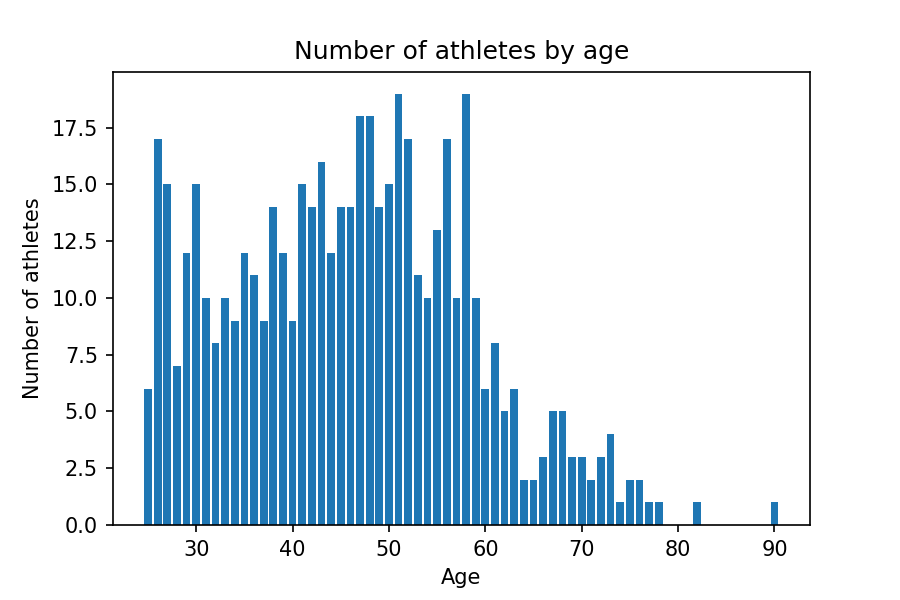
\includegraphics[width=\textwidth]{img/athletesbyage}
    \caption{Number of athletes by age}
    \label{fig:athletesbyage}
\end{figure}

\subsection{Number of Athletes by Nation}\label{subsec:number-of-athletes-by-nation}

To determine the number of athletes by nation, we can run the following SQL query:

\begin{minted}{sql}
SELECT COUNT(*) nationCount, nation
FROM annp_final.athlete
GROUP BY nation
ORDER BY nationCount ASC;
\end{minted}

We can then plot the result, as illustrated in \cref{fig:athletesbynation}.

\begin{figure}[H]
    \centering
    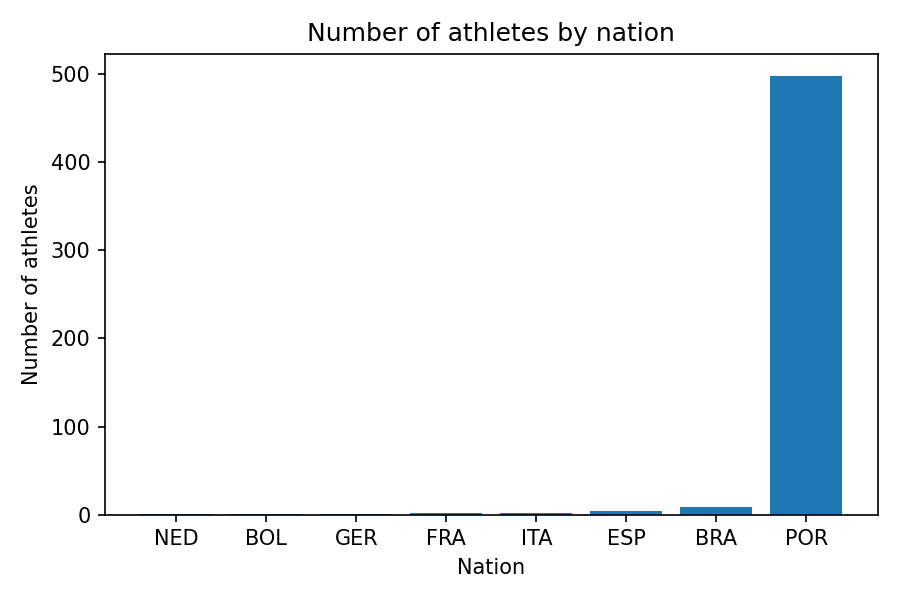
\includegraphics[width=.8\textwidth]{img/athletesbynation}
    \caption{Number of athletes by nation}
    \label{fig:athletesbynation}
\end{figure}

\subsection{Number of Athletes by Gender}\label{subsec:number-of-athletes-by-gender}

To determine the number of athletes by gender, we can run the following SQL query:

\begin{minted}{sql}
SELECT COUNT(*), gender
FROM annp_final.athlete
GROUP BY gender;
\end{minted}

We can then plot the result, as illustrated in \cref{fig:athletesbygender}.

\begin{figure}[H]
    \centering
    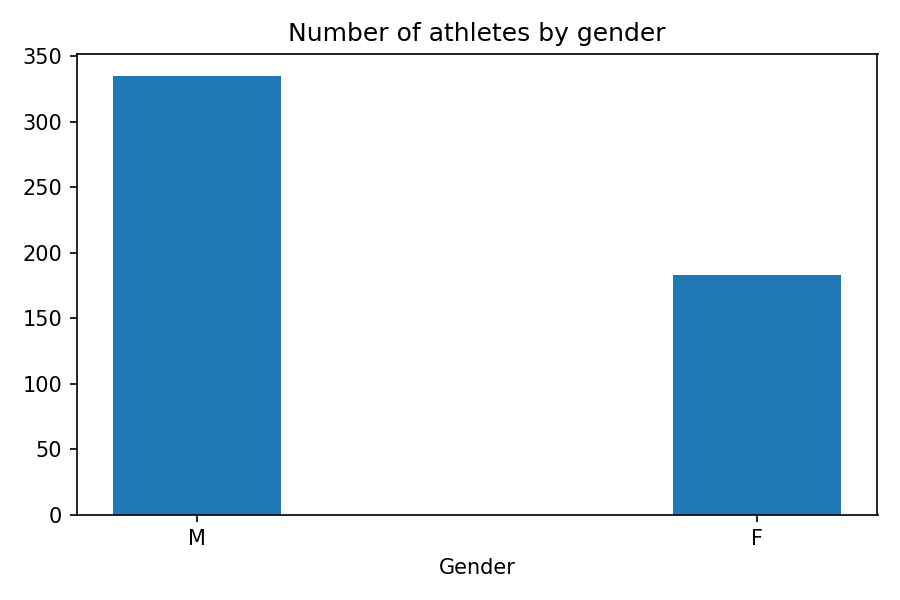
\includegraphics[width=.4\textwidth]{img/athletesbygender}
    \caption{Number of athletes by gender}
    \label{fig:athletesbygender}
\end{figure}

\subsection{Number of Events by Gender}\label{subsec:number-of-events-by-gender}

To determine the number of events by gender, we can run the following SQL query:

\begin{minted}{sql}
SELECT COUNT(*), gender
FROM annp_final.event
GROUP BY gender;
\end{minted}

We can then plot the result, as illustrated in \cref{fig:eventsbygender}.

\begin{figure}[H]
    \centering
    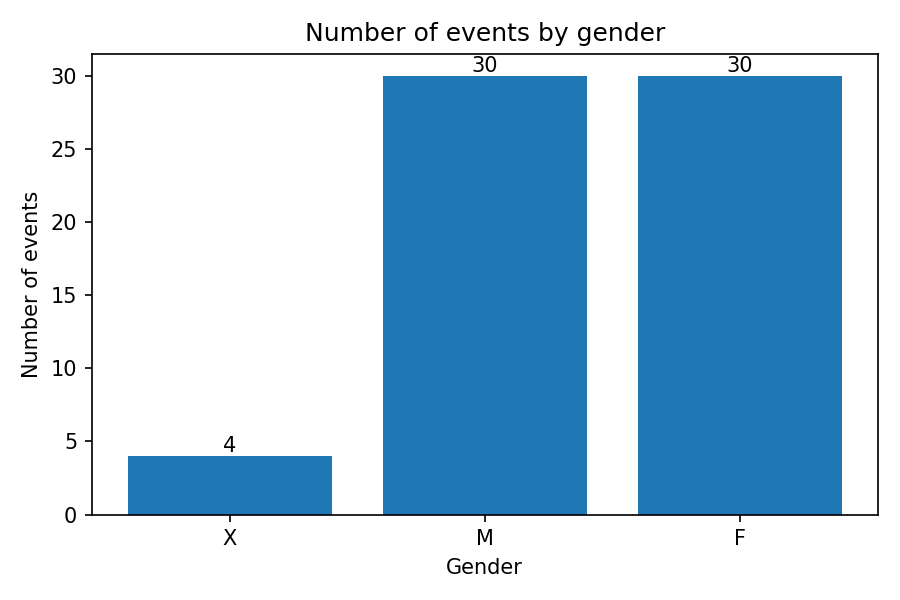
\includegraphics[width=.4\textwidth]{img/eventsbygender}
    \caption{Number of events by gender}
    \label{fig:eventsbygender}
\end{figure}

Here, the value \texttt{X} refers to events that allow athletes from both genders to participate.
